\subsubsection{Análisis Comparativo de Alternativas}

Para determinar la opción más adecuada de contenedor, se realizó un análisis comparativo detallado considerando aspectos técnicos, económicos y operativos de ambas alternativas.

\paragraph{Especificaciones del Contenedor Comercial Seleccionado}

Se identificó en el mercado nacional una canastilla plástica industrial con las siguientes características:

\begin{itemize}
    \item \textbf{Tipo}: Canastilla plástica 3/4 toda sellada de fábrica
    \item \textbf{Material}: Polipropileno industrial
    \item \textbf{Incluye}: Tapa
    \item \textbf{Capacidad de carga}: 200 kg
    \item \textbf{Costo unitario}: \$25,000 COP
    \item \textbf{Estado}: Nuevo, sellado de fábrica
\end{itemize}

Esta solución comercial fue comparada con la alternativa de fabricación propia mediante un análisis multicriterio.

\paragraph{Análisis de Costos}

La Tabla \ref{tab:costos_contenedor} presenta una comparación detallada de los costos asociados a cada alternativa para la fabricación de los 7 contenedores requeridos.

\begin{table}[H]
\centering
\caption{Comparación de costos entre alternativas de contenedor}
\label{tab:costos_contenedor}
\begin{tabular}{|l|r|r|}
\hline
\textbf{Concepto} & \textbf{Fabricación Propia} & \textbf{Contenedor Comercial} \\
\hline
\hline
\multicolumn{3}{|l|}{\textit{Materiales}} \\
\hline
Madera/MDF (láminas) & \$280,000 & --- \\
Herrajes y bisagras & \$105,000 & --- \\
Asas de transporte & \$42,000 & Incluidas \\
Tornillería & \$21,000 & --- \\
Adhesivos y sellantes & \$35,000 & --- \\
Pintura y acabados & \$70,000 & --- \\
Canastillas plásticas (7 unidades) & --- & \$175,000 \\
\hline
\textbf{Subtotal materiales} & \$553,000 & \$175,000 \\
\hline
\hline
\multicolumn{3}{|l|}{\textit{Procesos y mano de obra}} \\
\hline
Corte de materiales & \$140,000 & --- \\
Ensamblaje & \$210,000 & --- \\
Acabado superficial & \$105,000 & --- \\
\hline
\textbf{Subtotal procesos} & \$455,000 & \$0 \\
\hline
\hline
\multicolumn{3}{|l|}{\textit{Herramientas y equipos}} \\
\hline
Arriendo/depreciación herramientas & \$84,000 & --- \\
\hline
\textbf{Subtotal herramientas} & \$84,000 & \$0 \\
\hline
\hline
\textbf{COSTO TOTAL (7 unidades)} & \$1,092,000 & \$175,000 \\
\textbf{Costo unitario} & \$156,000 & \$25,000 \\
\hline
\end{tabular}
\end{table}

El análisis de costos revela una diferencia significativa de \$917,000 COP a favor de la opción comercial, lo que representa un ahorro del 84\% respecto a la fabricación propia.

\paragraph{Análisis de Tiempos}

La Tabla \ref{tab:tiempos_contenedor} compara los tiempos de implementación requeridos para cada alternativa.

\begin{table}[H]
\centering
\caption{Comparación de tiempos de implementación}
\label{tab:tiempos_contenedor}
\begin{tabular}{|l|r|r|}
\hline
\textbf{Actividad} & \textbf{Fabricación Propia} & \textbf{Contenedor Comercial} \\
\hline
Diseño detallado & 16 horas & 0 horas \\
Adquisición de materiales & 8 horas & 2 horas \\
Fabricación/corte & 24 horas & --- \\
Ensamblaje & 28 horas & --- \\
Acabados & 16 horas & --- \\
Curado y secado & 48 horas & --- \\
Inspección y ajustes & 8 horas & 1 hora \\
\hline
\textbf{TOTAL} & \textbf{148 horas} & \textbf{3 horas} \\
\textbf{Días laborales (8h/día)} & \textbf{18.5 días} & \textbf{0.4 días} \\
\hline
\end{tabular}
\end{table}

La opción comercial representa un ahorro de 145 horas de trabajo, equivalente a aproximadamente 18 días laborales, permitiendo dedicar este tiempo a otras actividades críticas del proyecto.

\paragraph{Análisis Técnico Comparativo}

La Tabla \ref{tab:comparativo_tecnico} presenta una evaluación de los aspectos técnicos y funcionales de ambas alternativas.

\begin{table}[H]
\centering
\caption{Análisis técnico comparativo de alternativas de contenedor}
\label{tab:comparativo_tecnico}
\small
\begin{tabular}{|p{4cm}|p{5cm}|p{5cm}|}
\hline
\textbf{Criterio} & \textbf{Fabricación Propia} & \textbf{Contenedor Comercial} \\
\hline
\hline
\textbf{Capacidad de carga} & 150-180 kg (estimado, requiere refuerzos) & 200 kg (certificado) \\
\hline
\textbf{Resistencia a apilamiento} & Variable, depende de la construcción & Certificada para apilamiento industrial \\
\hline
\textbf{Resistencia a humedad} & Requiere sellado y mantenimiento periódico & Resistente, material impermeable \\
\hline
\textbf{Durabilidad} & 3-5 años con mantenimiento & 10+ años, sin mantenimiento \\
\hline
\textbf{Peso del contenedor} & 8-12 kg (madera/MDF) & 3-4 kg (plástico) \\
\hline
\textbf{Transportabilidad} & Limitada por peso y volumen & Excelente, liviano con asas integradas \\
\hline
\textbf{Estandarización} & Cada unidad puede variar ligeramente & Todas las unidades idénticas \\
\hline
\textbf{Mantenimiento} & Requiere repintado, ajuste de herrajes & Mínimo, solo limpieza \\
\hline
\textbf{Reemplazo} & Difícil, requiere fabricación nueva & Inmediato, disponible en mercado \\
\hline
\textbf{Personalización} & Alta, diseño completamente adaptable & Limitada a dimensiones estándar \\
\hline
\textbf{Estética} & Profesional con buen acabado & Industrial, funcional \\
\hline
\end{tabular}
\end{table}

\paragraph{Matriz de Decisión}

Para la selección final se empleó una matriz de decisión multicriterio ponderada (Tabla \ref{tab:matriz_decision}), asignando pesos a cada criterio según su importancia relativa en el contexto del proyecto.

\begin{table}[H]
\centering
\caption{Matriz de decisión multicriterio para selección de contenedor}
\label{tab:matriz_decision}
\begin{tabular}{|l|c|c|c|c|c|}
\hline
\textbf{Criterio} & \textbf{Peso} & \multicolumn{2}{c|}{\textbf{Fabricación Propia}} & \multicolumn{2}{c|}{\textbf{Contenedor Comercial}} \\
\cline{3-6}
 & (\%) & Calif. & Pond. & Calif. & Pond. \\
\hline
Costo & 25 & 4 & 1.00 & 10 & 2.50 \\
Tiempo de implementación & 20 & 3 & 0.60 & 10 & 2.00 \\
Capacidad de carga & 15 & 7 & 1.05 & 9 & 1.35 \\
Durabilidad & 15 & 6 & 0.90 & 9 & 1.35 \\
Facilidad de transporte & 10 & 5 & 0.50 & 9 & 0.90 \\
Disponibilidad & 10 & 4 & 0.40 & 10 & 1.00 \\
Mantenimiento & 5 & 5 & 0.25 & 10 & 0.50 \\
\hline
\textbf{TOTAL} & \textbf{100} & --- & \textbf{4.70} & --- & \textbf{9.60} \\
\hline
\end{tabular}
\end{table}

\textit{Nota: Calificación en escala de 1 a 10, donde 10 es el mejor desempeño.}

\paragraph{Conclusión del Análisis}

El análisis comparativo multicriterio demostró que la opción de contenedor comercial (canastilla plástica industrial) es significativamente superior a la fabricación propia, obteniendo una puntuación ponderada de 9.60 frente a 4.70.

Las ventajas decisivas del contenedor comercial son:

\begin{enumerate}
    \item \textbf{Ventaja económica}: Ahorro de \$917,000 COP (84\%) en el costo total de los 7 contenedores
    \item \textbf{Ventaja temporal}: Reducción de 18 días laborales en el tiempo de implementación
    \item \textbf{Ventaja técnica}: Capacidad de carga certificada de 200 kg, superior a la estimada para fabricación propia
    \item \textbf{Ventaja operativa}: Menor peso (3-4 kg vs 8-12 kg), facilitando el transporte manual
    \item \textbf{Ventaja de mantenimiento}: Material resistente a humedad sin requerimiento de mantenimiento periódico
    \item \textbf{Ventaja de disponibilidad}: Reemplazo inmediato en caso de daño o necesidad de unidades adicionales
\end{enumerate}

La única ventaja de la fabricación propia sería la personalización completa del diseño; sin embargo, esta ventaja no compensa las múltiples desventajas en costo, tiempo, y características técnicas.

Por estas razones, se seleccionó la canastilla plástica industrial como contenedor definitivo para los 7 kits del proyecto, permitiendo una implementación más rápida, económica y técnicamente superior, liberando recursos financieros y temporales que pueden ser destinados a otros componentes críticos del kit de clasificación.


    \begin{figure}[H]
        \centering
        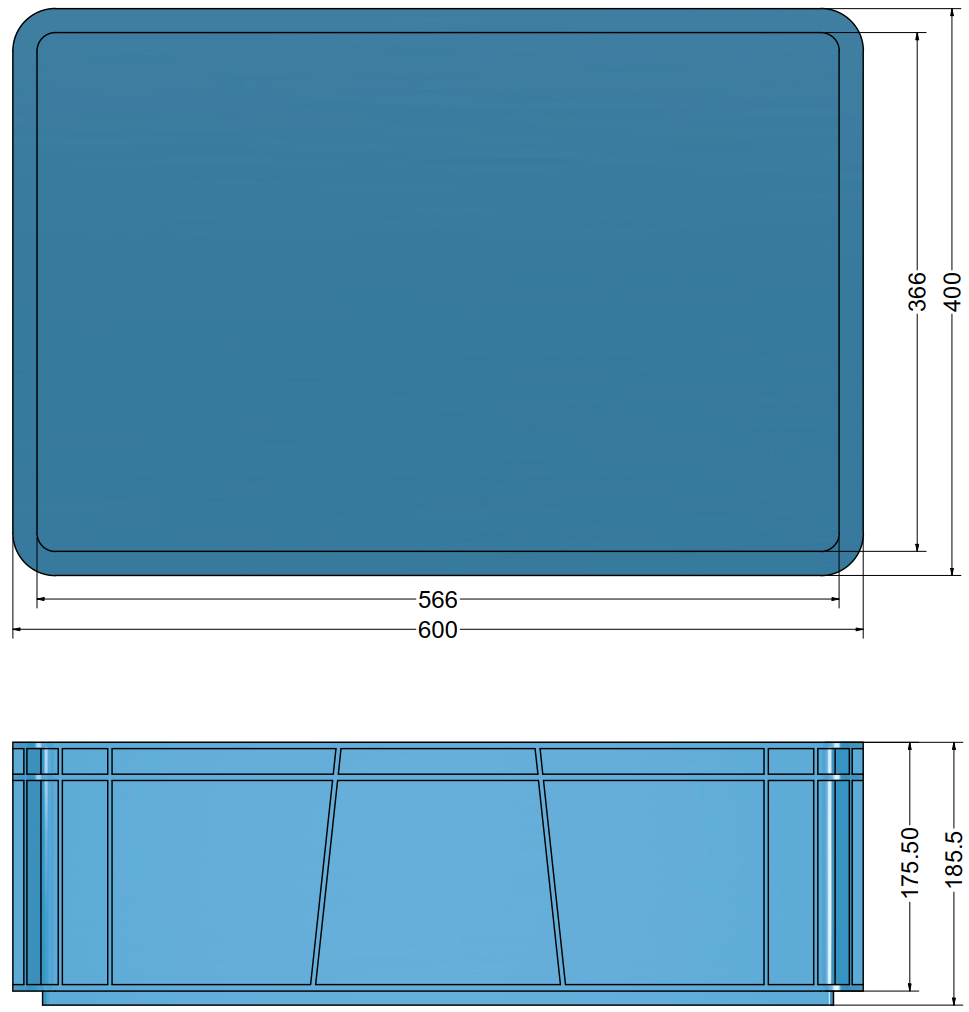
\includegraphics[width=0.9\textwidth]{06disenoConceptual/img/carcasa.png}
        \caption{Vista superior y lateral de canastilla 3/4 sellada con dimensiones externas e internas.}
        \label{fig:carcasa}
    \end{figure}
    
    
